\documentclass[11pt]{article}

% =========================
% Packages
% =========================
\usepackage[margin=0.78in]{geometry}
\usepackage{amsmath,amssymb,amsfonts,mathtools}
\usepackage{booktabs,array,tabularx,longtable,multirow}
\usepackage{enumitem}
\usepackage[most]{tcolorbox}
\usepackage{xcolor}
\usepackage{fancyhdr}
\usepackage{titlesec}
\usepackage{hyperref}
\usepackage{lastpage}
\usepackage{setspace}
\usepackage{tikz}
\usepackage{pgfplots}
\usepackage{needspace}
\usepackage{caption}
\usepackage{multicol}
\usepackage{graphicx}
\usepackage{amsthm}
\usepackage{mathrsfs}
\usepackage{bm}
\usepackage{float}
\usepackage{changepage}
\usetikzlibrary{calc,arrows.meta,positioning,decorations.pathreplacing,patterns,angles,quotes}

\pgfplotsset{compat=1.18}
\setstretch{1.14}
\setlength{\parindent}{0pt}
\setlength{\parskip}{0.45em}
\setlist[itemize]{leftmargin=1.8em}
\setlist[enumerate]{leftmargin=2em}

% =========================
% Colors
% =========================
\definecolor{novelPurple}{RGB}{98,54,255}
\definecolor{novelPurpleDark}{RGB}{72,34,204}
\definecolor{novelPurpleLight}{RGB}{243,239,255}
\definecolor{novelPurpleLine}{RGB}{165,135,255}
\definecolor{npgray}{RGB}{78,78,78}
\definecolor{softgray}{RGB}{246,246,250}
\definecolor{softlav}{RGB}{249,247,255}
\definecolor{greencheck}{RGB}{24,128,88}
\definecolor{warmred}{RGB}{188,54,54}
\definecolor{nporange}{RGB}{223,121,36}
\definecolor{npgreen}{RGB}{67,142,103}
\definecolor{npred}{RGB}{180,54,54}

% =========================
% Hyperref
% =========================
\hypersetup{
    colorlinks=true,
    linkcolor=novelPurpleDark,
    urlcolor=novelPurpleDark,
    citecolor=novelPurpleDark
}

% =========================
% Header / Footer
% =========================
\pagestyle{fancy}
\fancyhf{}
\fancyhead[L]{\textbf{Novel Prep Learning Center}}
\fancyhead[R]{\textbf{AP Calculus AB --- Unit 3}}
\fancyfoot[C]{\textcolor{novelPurpleDark}{\thepage\ /\ \pageref{LastPage}}}
\renewcommand{\headrulewidth}{0.4pt}
\renewcommand{\footrulewidth}{0pt}

% =========================
% Section styles
% =========================
\setcounter{secnumdepth}{3}
\setcounter{tocdepth}{3}

\titleformat{\section}
{\Large\bfseries\color{novelPurpleDark}}{\thesection.}{0.6em}{}

\titleformat{\subsection}
{\large\bfseries\color{novelPurple}}{\thesubsection.}{0.6em}{}

\titleformat{\subsubsection}
{\normalsize\bfseries\color{novelPurpleDark}}{\thesubsubsection.}{0.6em}{}

% =========================
% Boxes
% =========================
\tcbset{enhanced,sharp corners,boxrule=1pt}

\newtcolorbox{theorybox}[1]{
  colback=white,
  colframe=novelPurple,
  colbacktitle=novelPurple,
  coltitle=white,
  title=\textbf{#1},
  fonttitle=\bfseries,
  sharp corners,
  breakable
}

\newtcolorbox{notebox}[1]{
  colback=novelPurpleLight,
  colframe=novelPurple,
  colbacktitle=novelPurple,
  coltitle=white,
  title=\textbf{#1},
  fonttitle=\bfseries,
  sharp corners,
  breakable
}

\newtcolorbox{skillbox}[1]{
  colback=softlav,
  colframe=novelPurpleDark,
  colbacktitle=novelPurpleDark,
  coltitle=white,
  title=\textbf{#1},
  fonttitle=\bfseries,
  sharp corners,
  breakable
}

\newtcolorbox{summarybox}[1]{
  colback=softgray,
  colframe=novelPurpleDark,
  colbacktitle=novelPurpleDark,
  coltitle=white,
  title=\textbf{#1},
  fonttitle=\bfseries,
  sharp corners,
  breakable
}

\newtcolorbox{practicebox}[1]{
  colback=white,
  colframe=novelPurpleLine,
  colbacktitle=novelPurpleLine,
  coltitle=black,
  title=\textbf{#1},
  fonttitle=\bfseries,
  sharp corners,
  breakable
}

% =========================
% Commands
% =========================
\newcounter{examplectr}[subsection]
\renewcommand{\theexamplectr}{\thesubsection.\arabic{examplectr}}

\newcommand{\example}[1]{%
\refstepcounter{examplectr}
\Needspace{8\baselineskip}
\noindent{\color{novelPurpleDark}\textbf{Example \theexamplectr.}} \textbf{#1}\par
}

\newcommand{\solution}{\noindent{\textbf{Solution.}}}
\newcommand{\unitchapter}[1]{\newpage\subsection{#1}}
\newcommand{\unitsubtopic}[1]{\subsubsection{#1}}

% =========================
% Figures
% =========================
\newcommand{\unitthreecoverfigure}{
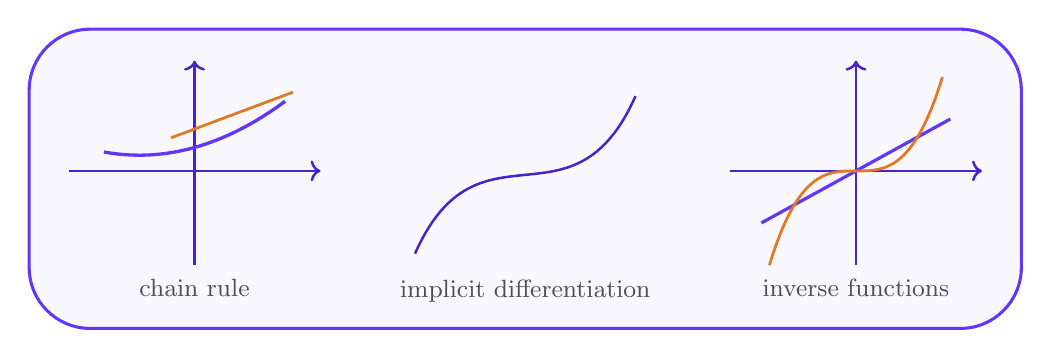
\begin{tikzpicture}[scale=1]
\fill[softlav,rounded corners=22pt] (-6.3,-1.9) rectangle (6.3,1.9);
\draw[novelPurple, line width=1.1pt, rounded corners=22pt] (-6.3,-1.9) rectangle (6.3,1.9);

\begin{scope}[shift={(-4.2,0.1)}]
\draw[novelPurpleDark, line width=0.9pt, ->] (-1.6,0)--(1.6,0);
\draw[novelPurpleDark, line width=0.9pt, ->] (0,-1.2)--(0,1.4);
\draw[novelPurple, line width=1.2pt, smooth, samples=180, domain=-1.15:1.15]
plot (\x,{0.2*(\x+0.7)^2+0.2});
\draw[nporange, line width=1.0pt] (-0.3,0.42)--(1.25,1.0);
\node[text=npgray] at (0,-1.48) {\small chain rule};
\end{scope}

\begin{scope}[shift={(0,0.05)}]
\draw[novelPurpleDark, line width=0.9pt] (-1.4,-1.0) .. controls (-0.6,0.8) and (0.6,-0.8) .. (1.4,1.0);
\node[text=npgray] at (0,-1.48) {\small implicit differentiation};
\end{scope}

\begin{scope}[shift={(4.2,0.1)}]
\draw[novelPurpleDark, line width=0.9pt, ->] (-1.6,0)--(1.6,0);
\draw[novelPurpleDark, line width=0.9pt, ->] (0,-1.2)--(0,1.4);
\draw[novelPurple, line width=1.15pt, smooth, samples=160, domain=-1.2:1.2]
plot (\x,{0.55*\x});
\draw[nporange, line width=1.0pt, smooth, domain=-1.1:1.1, samples=160]
plot (\x,{0.9*\x^3});
\node[text=npgray] at (0,-1.48) {\small inverse functions};
\end{scope}

;
\end{tikzpicture}
}

\newcommand{\chainrulefigure}{
\begin{center}
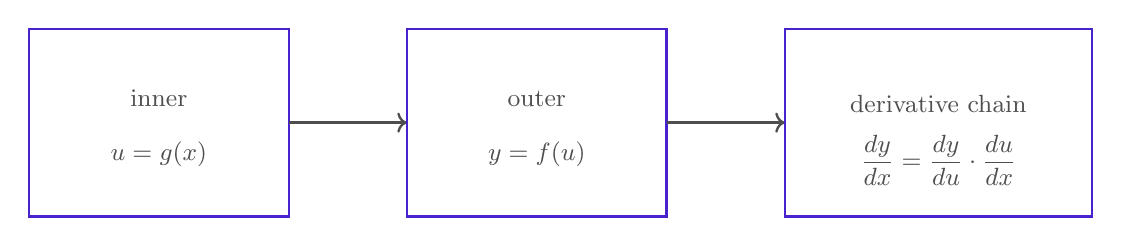
\begin{tikzpicture}[x=1.5cm,y=1.7cm]
    \draw[novelPurpleDark, line width=0.9pt] (0,0) rectangle (2.2,1.4);
    \node[text=npgray] at (1.1,0.88) {\small inner};
    \node[text=npgray] at (1.1,0.46) {\small $u=g(x)$};

    \draw[->, line width=0.85pt, npgray] (2.2,0.7)--(3.2,0.7);

    \draw[novelPurpleDark, line width=0.9pt] (3.2,0) rectangle (5.4,1.4);
    \node[text=npgray] at (4.3,0.88) {\small outer};
    \node[text=npgray] at (4.3,0.46) {\small $y=f(u)$};

    \draw[->, line width=0.85pt, npgray] (5.4,0.7)--(6.4,0.7);

    \draw[novelPurpleDark, line width=0.9pt] (6.4,0) rectangle (9.0,1.4);
    \node[text=npgray] at (7.7,0.84) {\small derivative chain};
    \node[text=npgray] at (7.7,0.42) {\small $\dfrac{dy}{dx}=\dfrac{dy}{du}\cdot\dfrac{du}{dx}$};
\end{tikzpicture}
\end{center}
}

\newcommand{\expchainfigure}{
\begin{center}
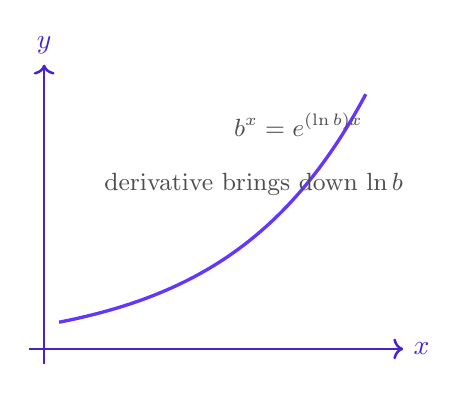
\begin{tikzpicture}[x=0.95cm,y=0.95cm]
\draw[novelPurpleDark, line width=0.9pt, ->] (-0.2,0)--(4.8,0) node[right] {$x$};
\draw[novelPurpleDark, line width=0.9pt, ->] (0,-0.2)--(0,3.8) node[above] {$y$};
\draw[novelPurple, line width=1.2pt, smooth, samples=200, domain=0.2:4.3]
plot (\x,{0.32*exp(0.55*\x)});
\node[text=npgray] at (3.4,3.0) {\small $b^x=e^{(\ln b)x}$};
\node[text=npgray] at (2.8,2.2) {\small derivative brings down $\ln b$};
\end{tikzpicture}
\end{center}
}

\newcommand{\implicitfigure}{
\begin{center}
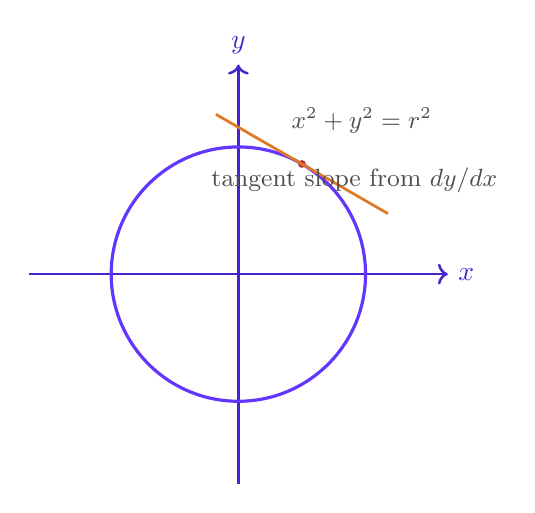
\begin{tikzpicture}[x=0.95cm,y=0.95cm]
    % axes
    \draw[novelPurpleDark, line width=0.9pt, ->] (-2.8,0)--(2.8,0) node[right] {$x$};
    \draw[novelPurpleDark, line width=0.9pt, ->] (0,-2.8)--(0,2.8) node[above] {$y$};

    % circle x^2 + y^2 = r^2, with r = 1.7
    \draw[novelPurple, line width=1.15pt] (0,0) circle (1.7);

    % label for equation
    \node[text=npgray] at (1.65,2.05) {\small $x^2+y^2=r^2$};

    % chosen point on the circle: angle 60 degrees
    \pgfmathsetmacro{\r}{1.7}
    \pgfmathsetmacro{\xp}{\r*cos(60)}
    \pgfmathsetmacro{\yp}{\r*sin(60)}

    % point on circle
    \fill[npred] (\xp,\yp) circle (1.4pt);

    % tangent line at (xp, yp)
    % for x^2+y^2=r^2, slope = -x/y
    \pgfmathsetmacro{\m}{-\xp/\yp}

    % draw tangent line using point-slope form
    \draw[nporange, line width=1.0pt]
        ({\xp-1.15},{\yp+\m*(-1.15)}) -- ({\xp+1.15},{\yp+\m*(1.15)});

    % tangent label
    \node[text=npgray] at (1.55,1.25) {\small tangent slope from $dy/dx$};
\end{tikzpicture}
\end{center}
}

\newcommand{\inversefigure}{
\begin{center}
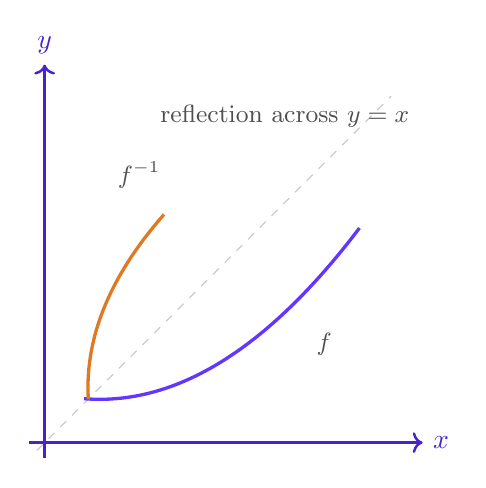
\begin{tikzpicture}[x=1cm,y=1cm]
\draw[novelPurpleDark, line width=0.9pt, ->] (-0.2,0)--(4.8,0) node[right] {$x$};
\draw[novelPurpleDark, line width=0.9pt, ->] (0,-0.2)--(0,4.8) node[above] {$y$};
\draw[gray!45,dashed] (-0.1,-0.1)--(4.4,4.4);
\draw[novelPurple, line width=1.2pt, smooth, samples=200, domain=0.5:4.0]
plot (\x,{0.2*(\x-0.7)^2+0.55});
\draw[nporange, line width=1.2pt, smooth, samples=200, domain=0.55:2.9]
plot ({0.2*(\x-0.7)^2+0.55},{\x});
\node[text=npgray] at (3.55,1.25) {\small $f$};
\node[text=npgray] at (1.2,3.4) {\small $f^{-1}$};
\node[text=npgray] at (3.05,4.15) {\small reflection across $y=x$};
\end{tikzpicture}
\end{center}
}

\newcommand{\higherorderfigure}{
\begin{center}
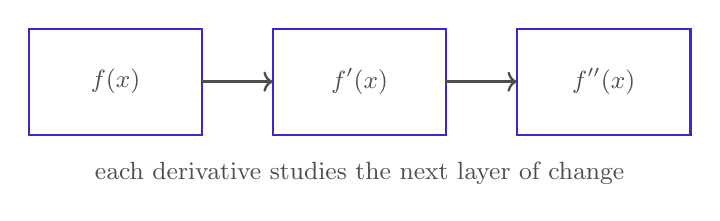
\begin{tikzpicture}[x=1cm,y=1cm]
\draw[novelPurpleDark, line width=0.9pt] (0,0) rectangle (2.2,1.35);
\node[text=npgray] at (1.1,0.68) {\small $f(x)$};
\draw[->, line width=0.85pt, npgray] (2.2,0.68)--(3.1,0.68);
\draw[novelPurpleDark, line width=0.9pt] (3.1,0) rectangle (5.3,1.35);
\node[text=npgray] at (4.2,0.68) {\small $f'(x)$};
\draw[->, line width=0.85pt, npgray] (5.3,0.68)--(6.2,0.68);
\draw[novelPurpleDark, line width=0.9pt] (6.2,0) rectangle (8.4,1.35);
\node[text=npgray] at (7.3,0.68) {\small $f''(x)$};
\node[text=npgray] at (4.2,-0.48) {\small each derivative studies the next layer of change};
\end{tikzpicture}
\end{center}
}

% =========================
% Document
% =========================
\begin{document}

\begin{titlepage}
\centering
\vspace*{1.9cm}

{\fontsize{28}{32}\selectfont\bfseries\color{novelPurpleDark} AP Calculus AB\par}
\vspace{0.35cm}
{\fontsize{28}{32}\selectfont\bfseries\color{novelPurpleDark} Unit 3: Differentiation of Composite, Implicit, and Inverse Functions\par}



\vspace{1.0cm}
\unitthreecoverfigure

\vfill

\begin{minipage}{0.84\textwidth}
\begin{notebox}{Design Goals for This Revision}
\begin{itemize}
    \item Preserve the original Unit 3 flow: Chain Rule, general exponential functions, implicit differentiation, inverse-function derivatives, and higher-order derivatives.
    \item Rebuild the chapter in the same polished Novel Prep style used for the later optimized units.
    \item Keep the original theorems and major examples while improving explanation, structure, and page design.
    \item Add enough interpretation so students understand \emph{why} these derivative rules work, not just how to execute them.
    \item Make the chapter strong enough for both first instruction and AP Calculus AB review.
\end{itemize}
\end{notebox}
\end{minipage}

\vfill

{\large\textbf{Novel Prep Learning Center}}\\[0.25em]
{\large J. Z}


\end{titlepage}

\tableofcontents
\newpage

\setcounter{section}{2}
\section{Differentiation: Composite, Implicit, and Inverse Functions}

\begin{theorybox}{Big Idea}
Unit 3 extends basic derivative rules to situations where variables are layered, hidden, or reversed.
Students move from direct derivatives to three deeper ideas:
\[
\text{composition} \longrightarrow \text{implicit dependence} \longrightarrow \text{inverse relationships}.
\]
\end{theorybox}

\begin{notebox}{Teaching Philosophy for This Unit}
Students should not see the Chain Rule, implicit differentiation, and inverse-function differentiation as unrelated tricks.
They all answer the same core question:
\begin{center}
\emph{If quantities depend on one another through multiple layers, how does the derivative track that dependence?}
\end{center}
This unit becomes much easier once students recognize that the derivative follows the structure of dependence.
\end{notebox}

\begin{summarybox}{AP Checkpoint}
The chapter naturally unfolds in four layers:
\begin{itemize}
    \item Composite structure: the Chain Rule
    \item Hidden dependence: implicit differentiation
    \item Reversed dependence: inverse functions
    \item Repeated differentiation: higher-order derivatives
\end{itemize}
\end{summarybox}

% =========================================================
\unitchapter{Chain Rule}

\unitsubtopic{The Main Rule}

\begin{theorybox}{Theorem 3.1.1 --- Chain Rule}
If $g$ is differentiable at $x$ and $f$ is differentiable at $g(x)$, then the composite function
\[
F=f\circ g,\qquad F(x)=f(g(x))
\]
is differentiable at $x$, and
\[
F'(x)=f'(g(x))\cdot g'(x).
\]
In Leibniz notation, if $y=f(u)$ and $u=g(x)$, then
\[
\frac{dy}{dx}=\frac{dy}{du}\cdot\frac{du}{dx}.
\]
\end{theorybox}

\chainrulefigure

\begin{notebox}{How to Read the Chain Rule}
The derivative of a composite function is:
\begin{center}
\emph{derivative of the outer function, evaluated at the inner function, times derivative of the inner function.}
\end{center}
A common student mistake is to differentiate only the outer layer and forget the inner derivative.
\end{notebox}

\begin{summarybox}{Quick Pattern Recognition}
If a function has the form
\[
[f(x)]^n,\qquad \sqrt{f(x)},\qquad e^{f(x)},\qquad \sin(f(x)),\qquad \ln(f(x)),
\]
then the Chain Rule is likely required because one function is sitting inside another.
\end{summarybox}
\newpage
\unitsubtopic{Comments on the Proof of the Chain Rule}

\noindent
Let
\[
\Delta u=g(x+\Delta x)-g(x).
\]
Then the corresponding change in $y=f(u)$ is
\[
\Delta y=f(u+\Delta u)-f(u).
\]
Informally, the proof idea is that the total rate of change from $x$ to $y$ is built by combining:
\begin{itemize}
    \item how $u$ changes with respect to $x$, and
    \item how $y$ changes with respect to $u$.
\end{itemize}
This is exactly why the derivative multiplies:
\[
\frac{dy}{dx}=\frac{dy}{du}\cdot\frac{du}{dx}.
\]

\example{Find the derivative of a composite radical function}
Find $F'(x)$ if
\[
F(x)=\sqrt{x^2+1}.
\]

\solution
Let
\[
f(u)=\sqrt{u},\qquad g(x)=x^2+1.
\]
Then
\[
F(x)=f(g(x)).
\]
Now
\[
f'(u)=\frac{1}{2\sqrt{u}},
\qquad
 g'(x)=2x.
\]
So by the Chain Rule,
\[
F'(x)=f'(g(x))\cdot g'(x)=\frac{1}{2\sqrt{x^2+1}}\cdot 2x.
\]
Thus
\[
\boxed{F'(x)=\frac{x}{\sqrt{x^2+1}}.}
\]

\example{Power Rule + Chain Rule + Quotient Rule together}
Find the derivative of
\[
g(t)=\left(\frac{t-2}{2t+1}\right)^9.
\]

\solution
Differentiate the outer power first:
\[
g'(t)=9\left(\frac{t-2}{2t+1}\right)^8\cdot\frac{d}{dt}\left(\frac{t-2}{2t+1}\right).
\]
Now use the Quotient Rule on the inner function:
\[
\frac{d}{dt}\left(\frac{t-2}{2t+1}\right)
=\frac{(2t+1)(1)-2(t-2)}{(2t+1)^2}.
\]
Simplify the numerator:
\[
(2t+1)-2t+4=5.
\]
So
\[
g'(t)=9\left(\frac{t-2}{2t+1}\right)^8\cdot\frac{5}{(2t+1)^2}.
\]
Therefore,
\[
\boxed{g'(t)=\frac{45(t-2)^8}{(2t+1)^{10}}.}
\]
\newpage
\unitsubtopic{Derivatives of General Exponential Functions}

\begin{theorybox}{Derivative of a General Exponential Function}
For any base $b>0$,
\[
b^x=e^{(\ln b)x}.
\]
Differentiating using the Chain Rule gives
\[
\frac{d}{dx}(b^x)=b^x\ln b.
\]
More generally, if the exponent is itself a function $u(x)$, then
\[
\frac{d}{dx}\bigl(b^{u(x)}\bigr)=b^{u(x)}\ln b\cdot u'(x).
\]
\end{theorybox}

\expchainfigure

\example{Differentiate basic and composite exponential functions}
Find the derivative of each function:
\begin{enumerate}
    \item $g(x)=2^x$
    \item $h(x)=5^{x^2}$
\end{enumerate}

\solution
\textbf{(a)} Using the formula with base $2$,
\[
g'(x)=2^x\ln 2.
\]

\textbf{(b)} Here the outer function is exponential and the inner function is $x^2$.
So,
\[
h'(x)=5^{x^2}\ln 5\cdot\frac{d}{dx}(x^2).
\]
Hence
\[
\boxed{h'(x)=2x\cdot 5^{x^2}\ln 5.}
\]

\begin{notebox}{Teacher Emphasis}
Students often memorize
\[
\frac{d}{dx}(a^x)=a^x\ln a
\]
but then forget to multiply by the inner derivative when the exponent is not just $x$.
\end{notebox}

% =========================================================
\unitchapter{Implicit Differentiation}

\unitsubtopic{Implicit and Explicit Functions}

\begin{theorybox}{Explicit vs. Implicit Form}
A function is in \textbf{explicit form} when the dependent variable is already solved for, such as
\[
y=3x^2-5.
\]
A function is in \textbf{implicit form} when the variables are mixed together in one equation, such as
\[
xy=1.
\]
In many cases, implicit form is easier to work with than solving explicitly for $y$.
\end{theorybox}

\begin{summarybox}{Example of the Difference}
\renewcommand{\arraystretch}{1.35}
\begin{tabularx}{\textwidth}{@{}p{0.26\textwidth}p{0.26\textwidth}X@{}}
\toprule
\textbf{Implicit Form} & \textbf{Explicit Form} & \textbf{Derivative}\\
\midrule
$xy=1$ & $y=\dfrac1x=x^{-1}$ & $\dfrac{dy}{dx}=-x^{-2}=-\dfrac1{x^2}$\\
\bottomrule
\end{tabularx}
\end{summarybox}

\noindent
Sometimes explicit form is easy to find, but in other cases it is difficult or impossible to solve nicely for $y$.
For example, the relation
\[
x^2-2y^3+4y=2
\]
is much better handled with implicit differentiation.
\newpage
\unitsubtopic{Differentiating with Respect to $x$}

\begin{theorybox}{Important Rule}
When differentiating with respect to $x$,
\[
\frac{d}{dx}[y^n]=ny^{n-1}\frac{dy}{dx}
\]
because $y$ depends on $x$.
\end{theorybox}

\begin{summarybox}{Mini Examples}
\begin{align*}
\frac{d}{dx}[x^3] &= 3x^2,\\
\frac{d}{dx}[y^3] &= 3y^2\frac{dy}{dx},\\
\frac{d}{dx}[x+3y] &= 1+3\frac{dy}{dx},\\
\frac{d}{dx}[xy^2] &= x\frac{d}{dx}(y^2)+y^2\frac{d}{dx}(x)
=2xy\frac{dy}{dx}+y^2.
\end{align*}
\end{summarybox}

\implicitfigure

\unitsubtopic{Implicit Differentiation Procedure}

\begin{skillbox}{Guidelines for Implicit Differentiation}
\begin{enumerate}
    \item Differentiate both sides of the equation with respect to $x$.
    \item Collect all terms involving $\dfrac{dy}{dx}$ on one side.
    \item Factor out $\dfrac{dy}{dx}$.
    \item Solve algebraically for $\dfrac{dy}{dx}$.
\end{enumerate}
\end{skillbox}

\example{Determine the slope of an implicit curve at a point}
Determine the slope of the graph of
\[
3(x^2+y^2)^2=100xy
\]
at the point $(3,1)$.

\solution
Differentiate both sides with respect to $x$:
\[
\frac{d}{dx}\bigl[3(x^2+y^2)^2\bigr]=\frac{d}{dx}[100xy].
\]
Using the Chain Rule on the left,
\[
3\cdot 2(x^2+y^2)\left(2x+2y\frac{dy}{dx}\right)=100\left(x\frac{dy}{dx}+y\right).
\]
So
\[
6(x^2+y^2)\left(2x+2y\frac{dy}{dx}\right)=100x\frac{dy}{dx}+100y.
\]
Expand:
\[
12x(x^2+y^2)+12y(x^2+y^2)\frac{dy}{dx}=100x\frac{dy}{dx}+100y.
\]
Collect the derivative terms on one side:
\[
12y(x^2+y^2)\frac{dy}{dx}-100x\frac{dy}{dx}=100y-12x(x^2+y^2).
\]
Factor out $\dfrac{dy}{dx}$:
\[
\left(12y(x^2+y^2)-100x\right)\frac{dy}{dx}=100y-12x(x^2+y^2).
\]
Thus
\[
\frac{dy}{dx}=\frac{100y-12x(x^2+y^2)}{-100x+12y(x^2+y^2)}.
\]
Now substitute $(x,y)=(3,1)$:
\[
\frac{dy}{dx}=\frac{100(1)-12(3)(3^2+1^2)}{-100(3)+12(1)(3^2+1^2)}
=\frac{100-36(10)}{-300+12(10)}
=\frac{-260}{-180}
=\frac{13}{9}.
\]
Therefore, the slope at $(3,1)$ is
\[
\boxed{\frac{13}{9}}.
\]

\begin{notebox}{Common Implicit-Differentiation Errors}
\begin{itemize}
    \item Forgetting to multiply by $\dfrac{dy}{dx}$ when differentiating a $y$-term
    \item Dropping product-rule terms such as $\dfrac{d}{dx}(xy)$
    \item Substituting the point before solving for $\dfrac{dy}{dx}$
\end{itemize}
\end{notebox}

% =========================================================
\unitchapter{Derivative of an Inverse Function}

\begin{theorybox}{Theorem 3.3.1 --- Derivative of an Inverse Function}
Let $f$ be invertible and differentiable, and let $y=f^{-1}(x)$ be its inverse.
If
\[
f'\bigl(f^{-1}(x)\bigr)\ne 0,
\]
then
\[
\frac{d}{dx}\bigl(f^{-1}(x)\bigr)=\frac{1}{f'\bigl(f^{-1}(x)\bigr)}.
\]
Equivalently, if $g(x)=f^{-1}(x)$, then
\[
g'(x)=\frac{1}{f'(g(x))}.
\]
\end{theorybox}

\inversefigure

\begin{summarybox}{Interpretation}
If $f$ and $f^{-1}$ are inverse functions, then their graphs are reflections across the line $y=x$.
A slope on one graph becomes the reciprocal slope on the reflected graph.
That is the geometric reason the derivative formula contains a reciprocal.
\end{summarybox}

\example{Find the derivative of an inverse function at a point}
Suppose
\[
f(x)=x^5+2x^3+7x+1.
\]
Find
\[
(f^{-1})'(1).
\]

\solution
Use the inverse-derivative formula:
\[
(f^{-1})'(1)=\frac{1}{f'(f^{-1}(1))}.
\]
So we first need to know $f^{-1}(1)$, which means we need the value of $x$ for which $f(x)=1$.
Observe that
\[
f(0)=0+0+0+1=1.
\]
So
\[
f^{-1}(1)=0.
\]
Now compute the derivative of $f$:
\[
f'(x)=5x^4+6x^2+7.
\]
Thus
\[
f'(0)=7.
\]
Therefore,
\[
\boxed{(f^{-1})'(1)=\frac17.}
\]

\begin{notebox}{Why This Formula Is Powerful}
The inverse function itself may be very difficult to write explicitly. The formula lets us compute the derivative of the inverse without ever solving for the inverse function.
\end{notebox}

% =========================================================
\unitchapter{Differentiating Inverse Functions}

\unitsubtopic{A Practical Method}

\begin{theorybox}{Practical Workflow}
To compute the derivative of an inverse function at a point:
\begin{enumerate}
    \item Identify the output value where the inverse derivative is requested.
    \item Solve $f(a)=b$ to find the corresponding input value $a$.
    \item Compute $f'(a)$.
    \item Take the reciprocal:
    \[
    (f^{-1})'(b)=\frac{1}{f'(a)}.
    \]
\end{enumerate}
\end{theorybox}

\example{Differentiate an inverse trig-style model without solving explicitly}
Let
\[
f(x)=x+\sin x.
\]
Assume $f$ is invertible on a suitable interval. Find
\[
(f^{-1})'(0).
\]

\solution
We need the value $a$ such that
\[
f(a)=0.
\]
Since
\[
f(0)=0+\sin 0=0,
\]
we have
\[
f^{-1}(0)=0.
\]
Now differentiate:
\[
f'(x)=1+\cos x.
\]
So
\[
f'(0)=1+1=2.
\]
Therefore,
\[
\boxed{(f^{-1})'(0)=\frac12.}
\]

\begin{summarybox}{Teacher Emphasis}
Students often try to solve explicitly for the inverse when it is unnecessary.
The correct habit is:
\[
\text{find the original input first, then evaluate } \frac{1}{f'(x)}.
\]
\end{summarybox}

% =========================================================
\unitchapter{Higher-Order Derivatives}

\begin{theorybox}{Higher-Order Derivatives}
The first derivative describes the rate of change of a function. The second derivative describes the rate of change of the first derivative, and so on.
We write:
\[
f''(x),\qquad f^{(3)}(x),\qquad f^{(4)}(x),\dots
\]
for higher-order derivatives.
\end{theorybox}

\higherorderfigure

\begin{notebox}{Why Higher-Order Derivatives Matter}
Even before Unit 5 and Unit 10, higher-order derivatives already matter because they help describe:
\begin{itemize}
    \item acceleration in motion,
    \item concavity of graphs,
    \item and the later structure of Taylor polynomials.
\end{itemize}
\end{notebox}

\example{Compute higher-order derivatives}
If
\[
y=x^4-3x^2+2x,
\]
find $y'$, $y''$, and $y^{(3)}$.

\solution
Differentiate repeatedly:
\[
y'=4x^3-6x+2,
\]
\[
y''=12x^2-6,
\]
\[
y^{(3)}=24x.
\]
So the derivatives are
\[
\boxed{y'=4x^3-6x+2,\qquad y''=12x^2-6,\qquad y^{(3)}=24x.}
\]

\example{Higher-order derivative with chain rule structure}
If
\[
y=e^{x^2},
\]
find $y'$ and $y''$.

\solution
First derivative:
\[
y'=e^{x^2}\cdot 2x=2xe^{x^2}.
\]
Differentiate again using the Product Rule:
\[
y''=2e^{x^2}+2x\bigl(e^{x^2}\cdot 2x\bigr).
\]
So
\[
y''=2e^{x^2}+4x^2e^{x^2}=2e^{x^2}(1+2x^2).
\]
Therefore,
\[
\boxed{y''=2e^{x^2}(1+2x^2).}
\]

% =========================================================
\newpage
\subsection{Unit 3 Summary / Formula Sheet}

\begin{summarybox}{Unit 3 Master Summary Sheet}
\renewcommand{\arraystretch}{1.35}
\begin{tabularx}{\textwidth}{@{}p{0.38\textwidth}X@{}}
\toprule
\textbf{Topic} & \textbf{Key Formula / Idea} \\
\midrule
Chain Rule & $(f\circ g)'(x)=f'(g(x))g'(x)$ \\
Leibniz notation & $\dfrac{dy}{dx}=\dfrac{dy}{du}\cdot\dfrac{du}{dx}$ \\
General exponential derivative & $\dfrac{d}{dx}(b^x)=b^x\ln b$ \\
Composite exponential derivative & $\dfrac{d}{dx}(b^{u(x)})=b^{u(x)}\ln b\cdot u'(x)$ \\
Implicit differentiation & differentiate both sides, collect $dy/dx$, solve \\
Derivative of inverse function & $(f^{-1})'(x)=\dfrac{1}{f'(f^{-1}(x))}$ \\
Inverse-function strategy & find original input first, then take reciprocal slope \\
Higher-order derivatives & $f''$, $f^{(3)}$, $f^{(4)}$, \dots \\
\bottomrule
\end{tabularx}
\end{summarybox}

\vspace{1em}

\begin{summarybox}{Big Strategy Ladder}
\begin{itemize}
    \item If one function is inside another, think Chain Rule.
    \item If $x$ and $y$ are mixed together, think implicit differentiation.
    \item If the function is reversed, think inverse derivative formula.
    \item If derivatives are repeated, organize the work carefully and differentiate one layer at a time.
\end{itemize}
\end{summarybox}

% =========================================================
\newpage
\subsection{Guided Practice Set}

\begin{practicebox}{Guided Practice A --- Chain Rule and Exponentials}
\begin{enumerate}
    \item Differentiate $y=(3x^2+1)^5$.
    \item Differentiate $y=\sqrt{1-x^3}$.
    \item Differentiate $y=4^{x^2+1}$.
    \item Explain in words how the Chain Rule follows the structure outer $\rightarrow$ inner.
\end{enumerate}
\end{practicebox}

\begin{practicebox}{Guided Practice B --- Implicit Differentiation}
\begin{enumerate}
    \item Find $\dfrac{dy}{dx}$ if $x^2+y^2=25$.
    \item Find $\dfrac{dy}{dx}$ if $xy+y^2=4$.
    \item Determine the slope of $x^2+xy+y^2=7$ at $(1,2)$.
    \item Explain why $\dfrac{d}{dx}[y^3]=3y^2\dfrac{dy}{dx}$.
\end{enumerate}
\end{practicebox}

\begin{practicebox}{Guided Practice C --- Inverse Functions and Higher Derivatives}
\begin{enumerate}
    \item If $f(2)=5$ and $f'(2)=8$, find $(f^{-1})'(5)$.
    \item If $f(1)=0$ and $f'(1)=3$, find $(f^{-1})'(0)$.
    \item Find the second derivative of $y=\sin(x^2)$.
    \item Explain why the slope of an inverse graph is the reciprocal of the original slope.
\end{enumerate}
\end{practicebox}

% =========================================================
\newpage
\subsection{Homework / Class Exercises}

\begin{practicebox}{Level 1 --- Skill Check}
\begin{enumerate}
    \item Differentiate $y=(x^2+4)^6$.
    \item Differentiate $y=\sqrt{2x+5}$.
    \item Differentiate $y=3^{x^2}$.
    \item Find $\dfrac{dy}{dx}$ if $x^2+y^2=9$.
    \item Find $y''$ if $y=x^3-2x^2+x$.
\end{enumerate}
\end{practicebox}

\begin{practicebox}{Level 2 --- AP Style Practice}
\begin{enumerate}
    \setcounter{enumi}{5}
    \item Differentiate $y=\left(\dfrac{x+1}{x-2}\right)^4$.
    \item Find the slope of the graph of $x^2-2y^3+4y=2$ at the point $(0,1)$.
    \item Suppose $f(0)=1$ and $f'(0)=7$. If $f$ is one-to-one, find $(f^{-1})'(1)$.
    \item If $y=e^{x^2+1}$, find $y'$ and $y''$.
    \item Explain the difference between explicit and implicit forms of a function.
\end{enumerate}
\end{practicebox}

\begin{practicebox}{Level 3 --- Challenge / Extension}
\begin{enumerate}
    \setcounter{enumi}{10}
    \item Show that the derivative of $\ln(f(x))$ is $\dfrac{f'(x)}{f(x)}$ using the Chain Rule.
    \item Find the equation of the tangent line to $x^2+y^2=25$ at the point $(3,4)$.
    \item If $f(2)=5$ and $f'(2)=\dfrac13$, find $(f^{-1})'(5)$ and interpret the result geometrically.
    \item Find the second derivative of $y=5^{x^2}$.
    \item Explain why implicit differentiation is often better than solving explicitly for $y$.
\end{enumerate}
\end{practicebox}

% =========================================================
\newpage
\subsection{Answer Key / Instructor Notes}

\begin{summarybox}{Selected Answers}
\begin{enumerate}
    \item $\dfrac{d}{dx}(x^2+4)^6=12x(x^2+4)^5$
    \item $\dfrac{d}{dx}\sqrt{2x+5}=\dfrac{1}{\sqrt{2x+5}}$
    \item $\dfrac{d}{dx}(3^{x^2})=2x\,3^{x^2}\ln 3$
    \item From $x^2+y^2=9$, $2x+2y\dfrac{dy}{dx}=0$, so $\dfrac{dy}{dx}=-\dfrac{x}{y}$
    \item If $y=x^3-2x^2+x$, then $y'=3x^2-4x+1$, $y''=6x-4$
    \item $\dfrac{d}{dx}\left(\dfrac{x+1}{x-2}\right)^4=4\left(\dfrac{x+1}{x-2}\right)^3\left(\dfrac{-3}{(x-2)^2}\right)$
    \item At $(0,1)$, implicit differentiation gives slope $0$
    \item $(f^{-1})'(1)=\dfrac{1}{f'(0)}=\dfrac17$
    \item If $y=e^{x^2+1}$, then $y'=2xe^{x^2+1}$ and $y''=2e^{x^2+1}(1+2x^2)$
    \item Explicit means $y$ is already isolated; implicit means $x$ and $y$ remain mixed in one equation
\end{enumerate}
\end{summarybox}

% =========================================================
\newpage
\subsection{Unit 3 Final Teaching Checklist}

\begin{summarybox}{Before Leaving Unit 3, Students Should Comfortably Handle}
\begin{itemize}
    \item identifying and differentiating composite functions with the Chain Rule
    \item differentiating general exponential functions with base $b$
    \item distinguishing explicit and implicit forms
    \item carrying out implicit differentiation correctly
    \item evaluating slopes of implicitly defined curves at specific points
    \item using the inverse-function derivative formula
    \item computing inverse derivatives without solving for the inverse explicitly
    \item finding and interpreting higher-order derivatives
    \item recognizing the structural theme connecting all of Unit 3
\end{itemize}
\end{summarybox}

\end{document}
